\section{问题一的模型建立与求解}
对于本问题情景,采用\textbf{贪心}的思想,参考操作系统进程调度的几种算法,考虑每完成一个订单后,如何选择下一个生产的订单,以达到总超时时间最小的目标。下面设计5种选择标准,形成5种算法进行求解:完成时间最短优先,剩余时间最短优先,完工截止时间最早、完成时间最短优先,完工截止时间最早、剩余时间最短优先,以及超时订单数最小、完成时间最短优先。所有算法的具体代码见附录。相应名词解释如下:
\begin{itemize}
    \item \textbf{完成时间}(\verb|sum_time|):完成订单所需要的时间,由每件产品的标准工时以及订单内容计算得到。
    \item \textbf{剩余时间}(\verb|rm_time|):若选择某订单,完成该订单后距离完工截止时间所剩的时间。
\end{itemize}

      \subsection{最短完成时间优先(msf)}
      本算法意在每次选择完成最快的订单作为下一个生产订单,以最小化平均等待时间或完成时间。最终所得总超时时间为2928861分钟。
      
      本算法的问题很明显,就是完成时间长的订单可能会一直等待,导致饥饿问题,使得超时时间过大。因此,本算法主要作为其他算法结果的参考。
      
      \subsection{最短剩余时间优先(erf)}
      本算法的核心思想是在多个待生产的订单中选择最紧迫的订单先完成,以解决长订单饥饿的问题,达到更优的公平性。
      最终所得总超时时间为2678287分钟。
      
      \subsection{最早完工截止时间、最短完成时间优先(dmsf)}
      针对最小化总超时时间的目标,采用\textbf{双贪心}策略,在mlf的基础上添加一个更高优先级的选择标准:完工截止时间最早,即根据完工截止时间将时间分段,在每段里优先生产短订单。
      最终所得总超时时间为2362896分钟。
      \subsection{最早完工截止时间、最短剩余时间优先(derf)}
      采用dmlf相同的思想,但在每个时间段里优先选择最紧迫的订单。
      最终所得总超时时间为2514299分钟。
      
      \subsection{最小超时订单数、最短完成时间优先(meonf)}
      采用\textbf{双贪心}策略。算法的核心思想是在每个完工截止时间到来时,选择使得超时订单最少的订单进行处理。第二贪心目标是订单的生产时间,即多个订单的最小期望超时数量相同时,短订单优先。
      最终所得总超时时间为2125455分钟。
      
      \subsection{结论与分析}
      最终meonf算法所得总超时时间最小,为2125455分钟。具体分配方案见附录\cref{tab:problem1}。下面从两个角度给出合理性解释。
      
      \subsubsection{最短完成时间优先}
      在每个完工截止时间即将到来时,可以证明,\textbf{将订单按所需生产时间从小到大的顺序处理,所得收益最大}。
      
      假设有一系列订单,编号为$1,2,\ldots,k,k+1$,每个订单的所需的生产时间为$a_1,a_2,\ldots,\\a_k,a_{k+1}$,其中$a_1 < a_2 < \cdots < a_k < a_{k+1}$。现将订单按所需生产时间从小到大排序,如\cref{fig:p1}所示。现在即将到达一个截止时间$t$,使得$k-1$号订单正好超时。此时的超时分钟数之和为
\begin{equation}
    \label{eq:p1} 
    T_1=3(a_1+a_2+\cdots+a_{k-1}-t)+2a_k+a_{k+1}
\end{equation}
      
\begin{figure}[h]
    \centering
    \begin{minipage}[c]{0.3\textwidth}
        \centering
        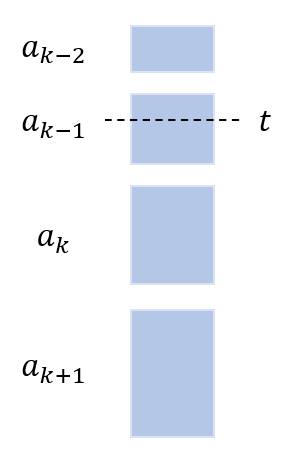
\includegraphics[height=0.2\textheight]{pics/p1.png}
        \subcaption{顺序排序}
        \label{fig:p1}
    \end{minipage} 
    \begin{minipage}[c]{0.3\textwidth}
        \centering
        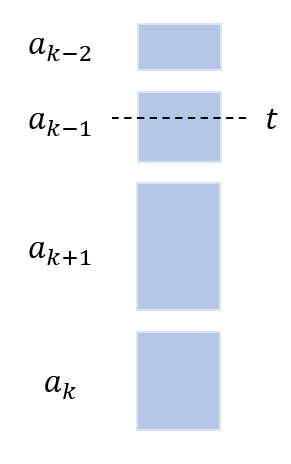
\includegraphics[height=0.2\textheight]{pics/p2.png}
        \subcaption{情况一}
        \label{fig:p2}
    \end{minipage} 
    \begin{minipage}[c]{0.3\textwidth}
        \centering
        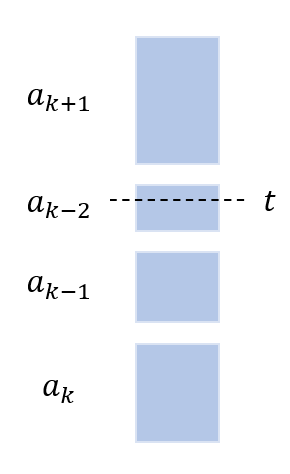
\includegraphics[height=0.2\textheight]{pics/p3.png}
        \subcaption{情况二}
        \label{fig:p3}
    \end{minipage} 
  \caption{不同订单处理顺序示意图}
  \label{fig:pro1}
\end{figure}
      
      若不按订单按所需生产时间从小到大排序处理,考虑将$k+1$号订单前移。可能有以下2种情况:
      
      \textbf{情况一}:若移动后的$k+1$号订单仍然超时,如\cref{fig:p2}所示。此时的超时分钟数之和为
\begin{equation}
    \label{eq:p2} 
    T_2=3(a_1+a_2+\cdots+a_{k-1}-t)+2a_{k+1}+a_k
\end{equation}

\cref{eq:p2}减去\cref{eq:p1},由于$a_k < a_{k+1}$,因此有
\[T_2-T_1=a_{k+1}-a_k>0\]

即总超时时间比顺序处理长。若移动后$k+1$号订单部分在截止时间内,类似可证超时时间增加。

\textbf{情况二}:若移动后的$k+1$号订单未超时,如\cref{fig:p3}所示。此时的超时分钟数之和为
\begin{equation}
    \label{eq:p3} 
    T_3=3(a_1+a_2+\cdots+a_{k-2}+a_{k+1}-t)+2a_{k-1}+a_k
\end{equation}

\cref{eq:p3}减去\cref{eq:p1},由于$a_{k-1} < a_k < a_{k+1}$,因此有
\[T_3-T_1=2a_{k+1}-a_k-a_{k-1}>0\]

即总超时时间比顺序处理长。其他情况均类似可证,在此不一一列举。因此,将长订单前移将增大总超时时间,故考虑将订单按所需生产时间从小到大的顺序处理具有合理性。
      
      \subsubsection{最小超时订单数优先}
       每次选择下一份订单时希望造成的超时订单数最少,是因为每多一个超时的订单,计算总超时时间的时候就要多一个累加对象,在短期看来效益较差。